\documentclass{llncs}


\usepackage{listings}
\usepackage{csquotes}
\usepackage{color}
\usepackage{caption}
\usepackage{graphicx}
\usepackage{zed}
\DeclareGraphicsExtensions{.pdf,.png,.jpg}
%%\newtheorem{definition}{Definition}
 \usepackage{listings}
 \usepackage{courier}
 \lstset{
         basicstyle=\footnotesize\ttfamily, % Standardschrift
         %numbers=left,               % Ort der Zeilennummern
         numberstyle=\tiny,          % Stil der Zeilennummern
         %stepnumber=2,               % Abstand zwischen den Zeilennummern
         numbersep=5pt,              % Abstand der Nummern zum Text
         tabsize=2,                  % Groesse von Tabs
         extendedchars=true,         %
         breaklines=true,            % Zeilen werden Umgebrochen
         keywordstyle=\color{red},
    		frame=b,         
 %        keywordstyle=[1]\textbf,    % Stil der Keywords
 %        keywordstyle=[2]\textbf,    %
 %        keywordstyle=[3]\textbf,    %
 %        keywordstyle=[4]\textbf,   \sqrt{\sqrt{}} %
         stringstyle=\color{white}\ttfamily, % Farbe der String
         showspaces=false,           % Leerzeichen anzeigen ?
         showtabs=false,             % Tabs anzeigen ?
         xleftmargin=17pt,
         framexleftmargin=17pt,
         framexrightmargin=5pt,
         framexbottommargin=4pt,
         %backgroundcolor=\color{lightgray},
         showstringspaces=false      % Leerzeichen in Strings anzeigen ?        
 }
 \lstloadlanguages{
         Java
 }
%\DeclareCaptionFont{blue}{\color{blue}} 

 %\captionsetup[lstlisting]{singlelinecheck=false, labelfont={blue}, textfont={blue}}
 % \usepackage{caption}
 
\DeclareCaptionFont{white}{\color{white}}
\DeclareCaptionFormat{listing}{\colorbox[cmyk]{0.43, 0.35, 0.35,0.01}{\parbox{\textwidth}{\hspace{15pt}#1#2#3}}}
 % \captionsetup[lstlisting]{format=listing,labelfont=white,textfont=white, singlelinecheck=false, margin=0pt, font={bf,footnotesize}}



\captionsetup[lstlisting]{format=listing,labelfont=white,textfont=white, singlelinecheck=false, margin=0pt, font={bf,footnotesize}}



\begin{document} 

\title{ISO11179 using Model Based Engineering}
%If Title is too long, use \titlerunning
%\titlerunning{Short Title}

%Single insitute
\author{David Milward \and Firstname Lastname}
%If there are too many authors, use \authorrunning
%\authorrunning{First Author et al.}
\institute{University of Oxford}
\maketitle

\begin{abstract}
In this paper we study how to implement an ISO11179 metadata registry using a data-oriented Domain Specific Modelling Language.  in particular we examine how certain weaknesses in the ISO specification can be strengthened by using a specific DSML built to handle interoperability user cases, and how using a model based engineering framework addresses allows many ambiguities in the standard to be decided and therefore implemented. We also examine how this DSL can fit into the EMF and UML frameworks, and what specific advantages are gained in using it to implement ISO11179. In particular we identify how MBE has helped in achieving the specific goals of ISO11179 which are given as: promoting the standard description of data; the common understanding of data across organisational elements and between organisations; the  re-use and standardisation of data over time, space, and applications; the harmonisation and standardisation of data within an organisation and across organisations; management of the components of data and lastly the re-use of the components of data.

\end{abstract}

\keywords{...}

\noindent

\section{Overview of ISO11179}

ISO11179 is the ISO standard for metadata registries. Metadata registries are used in many organisations to carry out a number of functions, nearly all of them are related to the need to ensure that data is used consistently within an organization.  The need for such a toolkit has become apparent in the last 10 years or so as the amount of data available to organizations has exploded, and despite the existence of an international standard metadata registries are implemented in a variety of different ways. In this paper we look at the intentions of the standard, and since there is no reference implementation of the standard we attempt to build an ISO11179 metadata registry using model driven engineering principles. During this process we examine the strengths and weaknesses of the standard and highlight areas in which the standard can be strengthened, made more user-friendly, adaptable and workable within an enterprise architectural framework. 


\subsection{The Purpose of ISO11179}

The ISO11179 Standard for metadata registries defines its purpose[REF]as follows,
\newline
to promote:
\begin{itemize}
\item Standard description of data
\item Common understanding of data across organizational elements and between organizations
\item Re-use and standardization of data over time, space, and applications
\item Harmonization and standardization of data within an organization and across organizations
\item Management of the components of data
\item Re-use of the components of data.
\end{itemize}

Interoperability isn't specifically mentioned, however these six items are very close to being a description of interoperability for data and data components. There is no other international standards which tackle the issues of interoperability, although there are a number of accepted ``'maturity models' which target interoperability (REF). These are similar in structure, address similar issues, but diverge slightly on implementation routes. The MDI model framework which emerged from the Athena and Interop NoE (REF) research projects have made progress in defining ways of implementing interoperability using model driven engineering concepts and ideas. Since ISO11179 is currently in use in both the Healthcare and Defence sectors it seems sensible to see if we can apply model driven interoperability concepts to implement the main features detailed in ISO11179, especially since no reference implementation of the standard is provided. It is also a chance to explore how these six use-cases are implemented by the standard and where such implementation is augmented by the use of Model Based Engineering techniques. Accordingly we have separate the paper into sections reflecting these core ISO11179 use cases.



\section{Standard Data Description}

The standard data description in ISO11179 is given in section1.6.1 where the idea of a data element is introduced, and with it the idea that it is composed of two parts, its conceptual part and its representational part. This section further puts forward the notion that a data element concept can be composed of two parts, an object class and a property. An object class is said to correspond with a class (in OO terms) or an entity(in ER terms). This is further illustrated with the illustration copied below:

\begin{figure}[h]
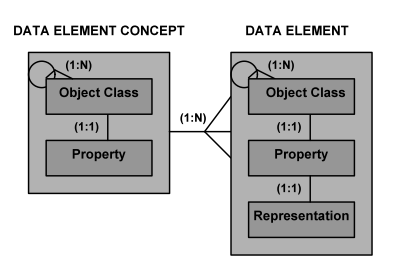
\includegraphics[width=0.7\textwidth,natwidth=610,natheight=642]{figs/DataElementConcept}
\caption{Data Elements and Data Element Concepts} 
\label{fig:DEC}
\end{figure}





\section{Common understanding of Data}


\section{Standardization of Data}


\section{Harmonization of Data Standards}


\section{Management of Data Components}


\section{Re-use of Data Components}

\section{Results}

\section{Discussion}

 


\newpage

\bibliographystyle{plain}

\bibliography{md11179}


\end{document}  